\documentclass[conference]{IEEEtran}
\IEEEoverridecommandlockouts
\usepackage{cite}
% fontspec + the Persian font must come BEFORE newtxtext (which breaks fontspec lookups under XeTeX)
\usepackage{fontspec}
\newfontfamily\persianfont[Script=Arabic]{Noto Naskh Arabic}
\TeXXeTstate=1
% Persian examples, right-to-left, in a font that has the glyphs
\newcommand{\fa}[1]{{\persianfont\beginR #1\endR}}
\usepackage{amsmath}
\usepackage{newtxtext}
\usepackage{newtxmath}
\usepackage{algorithm}
\usepackage{algorithmic}
\usepackage{graphicx}
\usepackage{booktabs}
\usepackage{tikz}
\usetikzlibrary{arrows.meta}
\usepackage{xcolor}
\usepackage[hidelinks]{hyperref}
% numbers still to be filled from output/research/*.json are marked \RES{}
% Every red number is traceable to research/PROGRESS.md. For the submission version replace the next
% line by \newcommand{\RES}[1]{#1} (all numbers then print in black).
\newcommand{\RES}[1]{\textcolor{red}{#1}}
\renewcommand{\algorithmicrequire}{\textbf{Input:}}
\renewcommand{\algorithmicensure}{\textbf{Output:}}

\begin{document}

\title{Training-Free Fixes for a Small CPU Persian Text-to-Speech Model:\\
Prompt Self-Extension for Short Utterances and Expressive Prosody for a Punctuation-Blind Model}

\author{\IEEEauthorblockN{AUTHOR-1, AUTHOR-2}
\IEEEauthorblockA{AFFILIATION\\ EMAIL}}

\maketitle

\begin{abstract}
Small continuous-latent text-to-speech (TTS) models now run in real time on a CPU, but short inputs are their
weak spot. We study a 110M-parameter Persian model and make three points. (i)~\emph{Measurement:} the usual
judge, Whisper, hallucinates on short audio; on real two-second recordings it fails \RES{17\%} of correct
clips. Scoring with two recognisers and counting a failure only when both agree, the true short-unit failure
rate is \RES{4--10\%}, five to ten times lower than Whisper alone reports. (ii)~\emph{Post-processing:}
signal checks the engine gets for free (energy, duration, end-of-speech timing, latent self- and
cross-similarity, syllable counts) predict which \emph{units} are risky but cannot tell a failed take from a
good take of the same unit, so retries without a recogniser recover little. (iii)~\emph{Pre-processing:}
failures depend on how the voice prompt \emph{ends}. We propose \emph{prompt self-extension}: once per
voice, the model reads one neutral sentence in that voice, and every later take is conditioned on the
reference clip followed by that reading. Ending the prompt at the model's own completed sentence is the
mechanism: cutting the extension mid-sentence multiplies failures by \RES{3--10}, and placing the clip last
makes the model read the extension aloud. On held-out short sentences rendered through the full production
pipeline with three voices, self-extension halves failed renders (\RES{24 $\to$ 12} of \RES{900}; consensus
error \RES{3.2\% $\to$ 2.2\%}, 95\% CI of the difference \RES{[$-$1.7, $-$0.4]} points) and raises UTMOS for
every voice; on three new, tightly cut real clips it cuts failures from \RES{96} to \RES{19} of \RES{450},
and a clip cut mid-clause goes from \RES{44\%} to \RES{3\%} error. The method needs no training and adds no per-request cost; its small
speaker-similarity cost on some voices disappears when the extension take is chosen by speaker similarity.
With it, the engine's retries can be dropped, halving the generation work while remaining more accurate.
(iv)~\emph{Intonation:} the model never sees punctuation, so a yes/no question is rendered sample-for-sample
like its statement twin. Restoring the contour after synthesis from the written mark --- a final rise
measured against real speech, applied by pitch-synchronous overlap-add --- moves the end of held-out yes/no
questions \RES{4.7} semitones above their statement twins (\RES{0.0} before; \RES{4.75} in real speech)
without new recognition failures, at the UTMOS cost of the signal processing (\RES{$-$0.24}).
(v)~\emph{Expressive prosody:} the voice prompt carries register and pitch range into the take, so we make
a livelier prompt from the model's own reading (re-pitched, widened, louder) and generate exclamations and
surprised questions from it; the audio rule keeps only the endings and the energy, and a loudness plan
spans the text. On held-out sentences, yes/no questions are heard as questions by a recogniser three times
as often (\RES{12\%} vs.\ \RES{4\%}), exclamations get a \RES{38\%} wider pitch range and \RES{2.2}\,dB more
level at almost no UTMOS cost (\RES{$-$0.02} vs.\ \RES{$-$0.24}), sentence loudness through a text varies
twice as much, and intelligibility is unchanged.
\end{abstract}

\begin{IEEEkeywords}
text-to-speech, Persian, robustness, voice prompt, inference-time methods, low-resource
\end{IEEEkeywords}

\section{Introduction}
Continuous audio language models (CALM) generate speech as a sequence of continuous codec latents
\cite{calm2025}; Pocket TTS distils such a model to a 100M-parameter student that runs faster than real
time on a laptop CPU \cite{pockettts2026}, and a community Persian student trained on 973\,h is available
\cite{farsiv2}. We use it, exported to ONNX, as the speech engine of a Persian--English assistant. Its
errors are not uniform: an assistant's short replies (\fa{«باشه»}, \fa{«ممنون از پیامتان»}) are exactly where it fails,
dropping final syllables or garbling the whole word.

\begin{figure*}[t]
\centering
% Fig. 1 — the engine and where each contribution sits (included with \input in main.tex)
\begin{tikzpicture}[x=1cm,y=1cm,font=\scriptsize,
  box/.style={draw=black!55,rounded corners=2pt,fill=black!4,align=center,minimum height=0.95cm,inner sep=2.5pt},
  ours/.style={box,draw=orange!80!black,fill=orange!14,line width=0.7pt},
  diag/.style={box,draw=black!45,fill=white,dashed},
  arr/.style={-{Stealth[length=1.6mm]},draw=black!70,line width=0.6pt},
  side/.style={-{Stealth[length=1.6mm]},draw=orange!80!black,line width=0.6pt},
  tag/.style={font=\tiny\bfseries,text=orange!70!black}]
% main row
\node[box,minimum width=1.75cm] (txt) at (0,0) {written text\\[-1pt]\fa{فایل را ذخیره کردید؟}};
\node[box,minimum width=2.05cm] (fe) at (2.55,0) {front end\\[-1pt]sentences, phrases\\[-1pt]\textbf{type} (\fa{؟}\,!\,.)};
\node[box,minimum width=1.9cm] (g2p) at (5.0,0) {G2P\\[-1pt]phonemes\\[-1pt]{\color{red!70!black}punctuation lost}};
\node[box,minimum width=2.15cm] (lm) at (7.6,0) {flow LM (110M)\\[-1pt]+ Mimi decoder\\[-1pt]one take per unit};
\node[box,minimum width=1.45cm] (join) at (10.05,0) {stitch \&\\[-1pt]join sentences};
\node[ours,minimum width=2.45cm] (into) at (12.5,0) {\textbf{sentence-type prosody}\\[-1pt]final rise / no fall,\\[-1pt]energy, loudness plan};
\node[box,minimum width=0.9cm] (out) at (14.6,0) {audio};
\draw[arr] (txt) -- (fe);
\draw[arr] (fe) -- (g2p);
\draw[arr] (g2p) -- (lm);
\draw[arr] (lm) -- (join);
\draw[arr] (join) -- (into);
\draw[arr] (into) -- (out);
% sentence type bypasses the model
\draw[side,dashed] (fe.north) -- ++(0,0.55) -| node[pos=0.25,above,font=\tiny,text=black!75]{sentence type kept in the text layer: question / wh-question / exclamation / statement} (into.north);
\node[tag,anchor=south east] at (into.north east) {C, D (Sec.~\ref{sec:c}, \ref{sec:d})};
% voice prompt row
\node[box,minimum width=1.75cm] (clip) at (2.55,-1.55) {reference clip\\[-1pt]($\le$5\,s, often cut tight)};
\node[ours,minimum width=3.15cm] (ext) at (6.0,-1.55) {\textbf{prompt self-extension}\\[-1pt]clip + model's own reading\\[-1pt]of one neutral sentence (once)};
\draw[arr] (clip) -- (ext);
\draw[side] (ext.north) -- node[right,font=\tiny,text=black!75,pos=0.45]{voice prompt} (ext.north |- lm.south) ;
\node[tag,anchor=north east] at (ext.south east) {B (Sec.~\ref{sec:b})};
% prosody-styled prompt (study D)
\node[ours,minimum width=3.4cm] (sty) at (6.0,-2.95) {\textbf{prosody-styled prompt}\\[-1pt]extension re-pitched, widened, louder\\[-1pt]per sentence type (built once)};
\draw[arr] (ext.south) -- (sty.north);
\draw[side] (sty.east) -| node[pos=0.75,right,font=\tiny,text=black!75]{livelier prompt for \fa{!}\,/\,\fa{؟}} ([xshift=0.35cm]lm.south);
\draw[side,dashed] ([xshift=-0.12cm]fe.south west) |- (sty.west);
\node[tag,anchor=north east] at (sty.south east) {D (Sec.~\ref{sec:d})};
% diagnosis and measurement
\node[diag,minimum width=2.4cm] (chk) at (10.05,-1.55) {take check without ASR\\[-1pt]finds risky \emph{units},\\[-1pt]not failed takes};
\draw[arr,dashed,draw=black!45] (lm.south east) ++(-0.2,0) |- (chk.west);
\node[tag,text=black!60,anchor=north east] at (chk.south east) {A (Sec.~\ref{sec:a})};
\node[diag,minimum width=2.5cm] (judge) at (13.1,-1.55) {evaluation: Whisper $\wedge$\\[-1pt]wav2vec2 consensus,\\[-1pt]F0 vs.\ real speech};
\draw[arr,dashed,draw=black!45] (out.south) |- (judge.east);
\end{tikzpicture}

\caption{The engine and the four studies. Orange: the inference-time fixes we propose --- prompt
self-extension before generation (B), sentence-type prosody after it (C, D), which uses the
punctuation the G2P discards, and a prosody-styled prompt chosen per sentence type (D). Dashed: the take check we show cannot replace a recogniser (A) and the
evaluation (two-recogniser consensus, F0 against real speech).}
\label{fig:pipeline}
\end{figure*}

Robustness of autoregressive TTS is usually bought with training: preference alignment and classifier-free
guidance \cite{koel2025}, fine-tuning on short phrases \cite{gepard2026}, or distilling ASR-verified
best-of-$N$ outputs back into the model \cite{asaria2026}. These need the training pipeline, data with
rights to use, and GPU time; for the released Persian student the 24-layer teacher it was distilled from is
not even public. We ask what can be done at inference time only (Fig.~\ref{fig:pipeline}), and answer four questions:

\begin{enumerate}
\item \textbf{Can post-processing catch failures without a recogniser?} We build a labelled corpus of
single takes and test every signal the engine sees for free. They identify risky units, not failed takes
(Sec.~\ref{sec:a}).
\item \textbf{Can the input be changed so the takes do not fail?} We show that how the voice prompt ends
drives short-unit failure and propose prompt self-extension, with an ordering rule that the model's
training explains (Sec.~\ref{sec:b}).
\item \textbf{Can a punctuation-blind model ask a question?} The model was trained on phonemes from which
every punctuation mark was removed; we show what it gets right from the words alone (wh-questions) and
restore what it cannot (yes/no questions, exclamations) after synthesis (Sec.~\ref{sec:c}).
\item \textbf{Can it sound surprised?} We show that the voice prompt carries register and pitch range, make
the expressive prompt from the model's own reading, and keep the signal processing to sentence endings
(Sec.~\ref{sec:d}).
\end{enumerate}
Answering both required fixing the measurement first: we show that a single ASR judge overstates short-unit
failures several-fold and use a two-recogniser consensus instead (Sec.~\ref{sec:system}).

\section{Related work}
\textbf{Robust AR TTS.} Hallucinated, repeated and dropped content is a known failure of autoregressive
TTS \cite{koel2025,borodin2026repetition}. Asaria et al.\ remove most catastrophic failures with ASR
self-verification and distillation \cite{asaria2026}; GEPARD reports a systematic collapse on 1--2-word
inputs and fixes it by fine-tuning \cite{gepard2026}; LEMAS penalises repetition during decoding
\cite{lemas2026}; LoopGuard detects loops from token diversity in text LLMs \cite{loopguard2026}. All
detectors we know of either use a recogniser or discrete tokens; a continuous-latent model has neither.

\textbf{Context at inference time.} For long-form speech, MagpieTTS-LF steers attention across chunks
\cite{magpielf2026}, Liu et al.\ post-train boundary-aware streaming \cite{liu2026boundary}, and Lim et al.\
find that the acoustic prompt must stay in context while speaker similarity still decays
\cite{lim2026longer}. We study the prompt itself: its length and what it ends with.

\textbf{Sentence type and intonation.} Vigneaux and Cole find that in English TTS a final question mark
is the only reliable lever on the nuclear tune, and steer tunes through the backbone's hidden state
\cite{vigneaux2026tunes}; Salem and Levitan find TTS systems under-produce rises on yes/no questions and
over-produce them on wh-questions \cite{salem2026question}; long prompts help reproduce a speaker's
intonation \cite{chen2026lptts}. Our model sees no punctuation at all and exposes no usable steering
direction (Sec.~\ref{sec:c}), so we restore the tune after synthesis, by classic TD-PSOLA \cite{psola1990}.
Expressiveness in zero-shot TTS is otherwise steered through the acoustic prompt: Expressive Prompting
selects emotionally intense prompts from a pool of recordings \cite{expprompt2026}, IndexTTS2 takes a style
prompt separate from the timbre prompt \cite{indextts2026}. Lacking expressive recordings of the target
speaker, we \emph{make} the expressive prompt from the model's own reading by signal processing; only the
prompt is processed, and the take is generated as usual (Sec.~\ref{sec:d}).
In Persian, yes/no questions end in a high boundary tone (H\%), while wh-questions fall like statements
with the nuclear accent on the question word \cite{sadat2011}.

\textbf{Persian TTS.} Open resources include ManaTTS \cite{manatts2025}, ParsVoice \cite{parsvoice2026},
homograph-aware G2P \cite{homorich2025} and the PARSA-Bench audio benchmark \cite{parsabench2026}.

\section{System and failure analysis}\label{sec:system}
\textbf{Model.} pocket-tts-farsi-v2 \cite{farsiv2} is a 6-layer CALM student (110M parameters) over 24\,kHz
Mimi \cite{moshi2024} latents at 12.5\,Hz. Text enters as Persian phonemes from a G2P model; English words are mapped to the
same phoneme set. Each unit is generated from a fresh state: \texttt{[BOS, voice prompt, text, latents\dots]}.
The voice prompt is a reference clip of at most 5\,s; in training it was the audio \emph{preceding} a random
word boundary of the same utterance, with the words after the boundary as text.

\textbf{Engine.} Text is split into sentences and phrases, then into units of at most 30 phoneme tokens by
dynamic programming over break costs (ezafe, verbs, \fa{«را»}). Each unit is generated up to three times; a
signal check (level, speech fraction, duration window, dead air) accepts a take or keeps the best of three.

\textbf{Corpus.} \RES{110} development sentences (short replies, casual, formal, numeric, mixed, English, long)
were planned exactly as in production, giving \RES{127} units; each was generated six times with each of three voices
(clips of 1.36\,s, 2.0\,s and 5.1\,s), without retries: \RES{2{,}286} takes. Each take is scored by
consonant-skeleton CER: consonants mapped to sound classes, vowels dropped on both sides, because Persian
script does not write short vowels.

\textbf{Two judges.} Whisper large-v3-turbo \cite{whisper2023} (beam 5, digits suppressed) is a poor judge of
short audio: on \RES{76} \emph{real} recordings of short Persian sentences (GPTInformal, CC0, mean
\RES{1.8}\,s) it charges skeleton CER \RES{0.188} and fails \RES{17\%} of them, often writing \fa{«موسیقی»}
(``music'') for speech. A character-level wav2vec2-CTC recogniser for Persian (no language model) fails
\RES{10.5\%} of the same clips (\RES{0.115}). On synthetic short takes the two judges correlate only
\RES{0.23}. We therefore report both and use a \emph{consensus} label: a take fails (CER $>0.3$) only if both
recognisers fail it, so a hallucination of either cannot fail a take. English units are judged by Whisper
alone.

\begin{figure}[t]
\centering
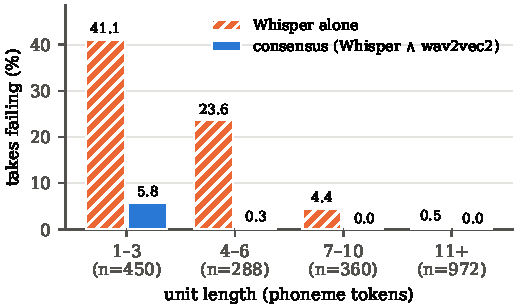
\includegraphics[width=\columnwidth]{figures/fig_judges.pdf}
\caption{Single-take failure rate (skeleton CER $>0.3$) by unit length on the development corpus
(\RES{2{,}070} Persian takes, three voices): Whisper alone vs.\ the two-recogniser consensus.}
\label{fig:judges}
\end{figure}

\textbf{Findings.} Under the consensus label \RES{1.3\%} of the \RES{2{,}070} Persian takes fail, all of
them in units of at most six phoneme tokens and nearly all in units of 1--3 tokens (\RES{5.8\%} of those
takes; none of the \RES{972} takes of more than ten tokens). Whisper alone would report \RES{12.3\%} overall
and \RES{41\%} for 1--3-token units (Fig.~\ref{fig:judges}). Most
failures are deletions (\RES{19} of \RES{27}), and the frames generated after end-of-speech are silent: the
model, not the trimming, drops the ending. Short-unit error depends on the voice prompt (\RES{0.060 / 0.027 /
0.016} for the 1.36 / 2.0 / 5.1\,s clips), and the two clips that ship with the engine end 0.02\,s and 0.07\,s
after their last phoneme.

\section{Post-processing without a recogniser}\label{sec:a}
A retry loop is only as good as its accept/reject test. We computed, for every take, the signals an engine
has for free.
\emph{Signal QC} (the engine's rule): level, fraction of frames with speech energy, speech duration against
a token-rate window, longest dead-air run.
\emph{Timing:} end-of-speech step per vowel of the target, speech seconds per vowel, the number of syllable
nuclei (peaks of the 0.3--2.5\,kHz envelope) against the number of vowels in the phonemes.
\emph{Latent recurrence:} the strongest off-diagonal stripe of the cosine self-similarity of the take's
latents over speech frames (0.64\,s window, lag $\ge$ 0.48\,s), which a take that says a stretch twice
produces; and the strongest stripe of its cross-similarity with the prompt's latents, which a take that
replays the prompt produces.
A logistic regression on these signals is trained on the development corpus and evaluated by
case-grouped cross-validation.

\textbf{Units, not takes.} With consensus labels the combined detector reaches a case-grouped
cross-validated AUC of \RES{0.88}, but its strongest input is the unit length itself (AUC \RES{0.94} alone).
Holding the unit fixed --- over all pairs of a failed and a good take of the same unit and voice --- the best
single signals reach \RES{0.66} (speech fraction) and \RES{0.67} (end-of-speech step per vowel), the engine's
rule \RES{0.58}, latent recurrence and prompt similarity \RES{0.48--0.57}. The signals know which units are
hard, not which take failed. They are not blind in general: on \RES{300} takes made with the clip placed
after the extension (Sec.~\ref{sec:b}), \RES{95\%} of which fail (the model reads the prompt's sentence), the prompt cross-similarity
separates them from normal takes of the same units with AUC \RES{0.98}. Natural failures of this engine are
different --- short deletions --- and those the signals do not see. The engine's rule is also badly calibrated: it rejects \RES{29\%} of takes,
\RES{96\%} of them good ones.

\textbf{Selection.} Table~\ref{tab:sel} replays retry policies on the six stored takes per unit. The
engine's rule spends \RES{49\%} more generation for \RES{2.35\%} $\to$ \RES{2.15\%} mean CER; keeping the
longest take (deletions dominate) or the latent DTW medoid does not help; an oracle choosing among the same
takes halves the error. The headroom exists, but finding it needs a recogniser. The held-out bench corpus (79 cases, four
takes per unit, \RES{1{,}632} Persian takes) repeats the picture: \RES{0.9\%} of takes fail, \RES{13} of
\RES{15} by deletion in units of $\le$6 tokens; the dev-trained detector falls to AUC \RES{0.78} and its
threshold does not transfer; retries move the error from \RES{2.89\%} to \RES{2.75\%} against an oracle's
\RES{1.23\%}. Since the failures sit in short units, we turn to the input.

\begin{table}[t]
\caption{Retry policies replayed on stored takes (dev, Persian, \RES{345} unit$\times$voice groups,
consensus CER / failure rate)}\label{tab:sel}
\centering
\begin{tabular}{lcc}
\toprule
policy & takes/unit & CER / fail \\
\midrule
first take & 1 & \RES{.0235 / 0.9\%} \\
engine signal QC (3 max) & \RES{1.49} & \RES{.0215 / 0.6\%} \\
ASR-free detector (3 max) & \RES{1.31} & \RES{.0251 / 1.2\%} \\
longest of 4 & 4 & \RES{.0236 / 0.9\%} \\
latent medoid of 3 & 3 & \RES{.0253 / 1.7\%} \\
oracle of 3 / of 6 & 3 / 6 & \RES{.0133 / 0.3\%}, \RES{.0114 / 0.3\%} \\
\bottomrule
\end{tabular}
\end{table}

\section{Prompt self-extension}\label{sec:b}
In training, the prompt is the audio that \emph{precedes} the target in the same recording, and the target
text starts after it. A reference clip that stops abruptly after its last phoneme --- as cleaned clips do ---
asks the model to continue an unfinished utterance with words it was not given, and short targets, which
leave the least room to recover, suffer most. We therefore extend the prompt with speech that the model
itself produces in the target voice and that ends the way training prompts end: at a completed sentence
(Fig.~\ref{fig:layout}).

\begin{figure}[t]
\centering
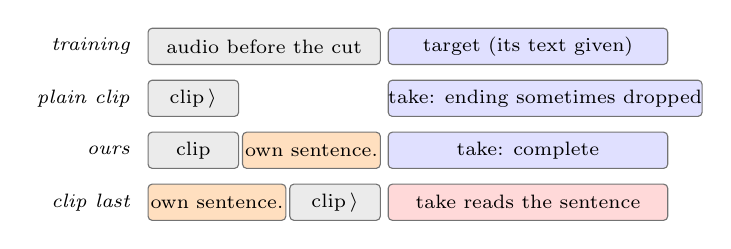
\begin{tikzpicture}[x=1cm,y=0.6cm,font=\scriptsize,
  b/.style={draw=black!55,rounded corners=1.5pt,minimum height=0.46cm,inner sep=0pt,align=center,anchor=west},
  lab/.style={anchor=east,font=\scriptsize\itshape}]
\node[lab] at (1.15,0) {training};
\node[b,fill=black!8,minimum width=2.95cm] at (1.25,0) {audio before the cut};
\node[b,fill=blue!12,minimum width=3.55cm] at (4.3,0) {target (its text given)};
\node[lab] at (1.15,-1.1) {plain clip};
\node[b,fill=black!8,minimum width=1.15cm] at (1.25,-1.1) {clip\,$\rangle$};
\node[b,fill=blue!12,minimum width=3.55cm] at (4.3,-1.1) {take: ending sometimes dropped};
\node[lab] at (1.15,-2.2) {ours};
\node[b,fill=black!8,minimum width=1.15cm] at (1.25,-2.2) {clip};
\node[b,fill=orange!25,minimum width=1.75cm] at (2.45,-2.2) {own sentence.};
\node[b,fill=blue!12,minimum width=3.55cm] at (4.3,-2.2) {take: complete};
\node[lab] at (1.15,-3.3) {clip last};
\node[b,fill=orange!25,minimum width=1.75cm] at (1.25,-3.3) {own sentence.};
\node[b,fill=black!8,minimum width=1.15cm] at (3.05,-3.3) {clip\,$\rangle$};
\node[b,fill=red!15,minimum width=3.55cm] at (4.3,-3.3) {take reads the sentence};
\end{tikzpicture}
\caption{Prompt layouts. In training the prompt is the audio preceding the target. A trimmed clip ends
mid-utterance ($\rangle$); prompt self-extension appends the model's own reading of a neutral sentence so
the prompt ends at a completed sentence. With the clip last, the model replays the extension.}
\label{fig:layout}
\end{figure}

\begin{algorithm}[t]
\caption{Prompt self-extension (once per voice)}\label{alg:ext}
\begin{algorithmic}[1]
\REQUIRE clip latents $c$ ($|c|\le 5$\,s), neutral sentence $s$, tries $K$
\FOR{$k=1..K$}
  \STATE $z_k \gets$ generate($s$ $\mid$ prompt $c$, seed $k$)
  \STATE $z_k \gets$ speech span of $z_k$ (+ one trailing frame)
\ENDFOR
\STATE $e \gets$ the $z_k$ of median speech length \COMMENT{no recogniser}
\STATE $p \gets [\,c \,;\, \text{last } (5\,\text{s} - |c|) \text{ of } e\,]$ \COMMENT{clip first, extension last}
\ENSURE prompt $p$, used for every later take of this voice
\end{algorithmic}
\end{algorithm}

The extension is kept as the model's own (normalised) latents, converted back to the codec space the
prompt is read in; decoding it to audio and re-encoding it worked less well in a Whisper-scored probe (\RES{0.286} vs
\RES{0.230} CER).
Choosing the take with a recogniser instead (lowest CER of the $K$) was not consistently
better (Table~\ref{tab:mech}); choosing it by speaker similarity is discussed below. The cost is $K$ short generations when a voice is added, and none per request: the extended prompt is
encoded once into the key--value cache that every unit already copies.

\textbf{Order.} With the clip placed \emph{after} the extension the prompt again ends abruptly, and the model
reads the extension sentence aloud instead of the text in \RES{94--99\%} of takes under both judges: the
take for the input \fa{«بله»} begins with \fa{«امروز هوا کمی سرد»}, the extension's opening words. The order
is therefore part of the method, not a detail.

\textbf{Controls.} Table~\ref{tab:mech} varies one thing at a time on the short development units
(180 paired takes per cell, consensus label). More real speech with the same abrupt ending (the clip twice)
does not help and hurts the male voice. The same extension cut after two thirds --- same voice, same kind of
latents, but ending mid-utterance --- multiplies failures by \RES{3--10} (Fig.~\ref{fig:ext}b). Teacher-forcing a carrier word
before the text (continuation priming) has no effect, and conditioning each unit on the previous unit's last
2\,s (to carry prosody across joins) adds nothing over the extension and, alone, lowers UTMOS by
\RES{0.11}. Which sentence is read matters: of seven candidates,
two (A, chosen first and fixed before any held-out test, and G) help both voices, whether the take is chosen
with or without a recogniser; three hurt the male voice, among them a greeting (B) and two neutral statements
(E, F). Neither the end-of-speech timing nor the engine's acceptance rate of the probe takes predicted which
sentences work (rank correlations from \RES{$-$0.06} to \RES{$-$0.58}, inconsistent across voices), so the
sentence is a hyperparameter that needs a judge to choose; we report this as a limitation rather than tune
it on test data. Sentence G, the other one that helped on development data, carries over only partly to the
held-out set (male voice \RES{$-$1.5} points, CI \RES{[$-$3.3, +0.1]}; female voice unchanged).

\begin{table}[t]
\caption{Prompt variants on short dev units: consensus CER (failed takes of 180)}\label{tab:mech}
\centering
\setlength{\tabcolsep}{4pt}
\begin{tabular}{lcc}
\toprule
prompt & male, 1.36\,s clip & female, 2.0\,s clip \\
\midrule
clip (baseline) & \RES{.075 (18)} & \RES{.033 (7)} \\
clip twice & \RES{.136 (27)} & \RES{.034 (8)} \\
clip + ext.\ A & \RES{.045 (8)} & \RES{.011 (2)} \\
clip + ext.\ A, ASR-free take & \RES{.037 (4)} & \RES{.021 (5)} \\
clip + ext.\ A cut mid-sentence & \RES{.229 (48)} & \RES{.333 (72)} \\
ext.\ A + clip (clip last) & \RES{1.33 (169)} & \RES{1.38 (179)} \\
clip + carrier \fa{«خب»} primed & \RES{.072 (16)} & \RES{.027 (5)} \\
clip + ext.\ B (greeting) & \RES{.148 (30)} & \RES{.038 (7)} \\
clip + ext.\ C (short replies) & \RES{.077 (16)} & \RES{.032 (6)} \\
clip + ext.\ D (formal) & \RES{.117 (28)} & \RES{.036 (8)} \\
clip + ext.\ A + B & \RES{.098 (17)} & \RES{.026 (8)} \\
clip + ext.\ E (neutral, past) & \RES{.102 (23)} & \RES{.027 (6)} \\
clip + ext.\ F (neutral, one clause) & \RES{.099 (23)} & \RES{.034 (7)} \\
clip + ext.\ G (neutral, habitual) & \RES{.043 (8)} & \RES{.019 (4)} \\
\bottomrule
\end{tabular}
\end{table}

\begin{figure*}[t]
\centering
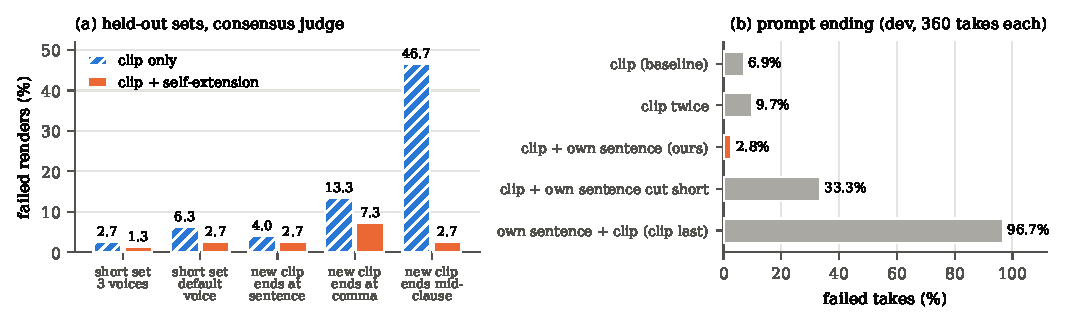
\includegraphics[width=\textwidth]{figures/fig_ext.pdf}
\caption{Prompt self-extension at a glance. (a) Failed renders (consensus judge) with the plain clip and with
the clip followed by the model's own reading of sentence A, on the held-out short set (pooled and for the
engine's default 1.36\,s voice) and for three new real clips cut 0.02\,s after their last sound: the less
finished the clip's ending, the larger the gain. (b) The mechanism on development units (male and female
voice pooled): ending the prompt at a completed sentence helps; the same extension cut short, or placed
before the clip, makes things worse.}
\label{fig:ext}
\end{figure*}

\textbf{Held-out results.} Two test sets were never used for any choice above (Fig.~\ref{fig:ext}a). \emph{Short:} 60 new
sentences of 1--5 words (50 Persian, 5 English, 5 mixed), rendered through the full production path (front
end, chunking, three-attempt signal retry, stitching). \emph{Bench:} 79 mixed cases (prose, numbers, dates,
English, code-mixed, acronyms, punctuation, 12 paragraphs). Table~\ref{tab:held} pairs renders by case and
seed. On short sentences, pooled over the three voices, failed renders halve (\RES{24 $\to$ 12} of
\RES{900} Persian renders; consensus error \RES{3.2\% $\to$ 2.2\%}, CI \RES{[$-$1.7, $-$0.4]} points). The
gain is significant for the 1.36\,s clip that the engine ships as its default (\RES{6.0\% $\to$ 3.9\%}) and
small for the two voices that were already near the floor. UTMOS \cite{utmos2022} rises for every voice
(\RES{+0.09 to +0.17}). Speaker similarity to the clip (WeSpeaker \cite{wespeaker2023}) is unchanged for both
male voices but drops by \RES{0.03} for the female voice, whose reading of the extension drifts from the
clip; this is the method's cost. On the bench, where most units are long, the final configuration also lowers the
Persian consensus error (\RES{2.9\% $\to$ 2.3\%}, CI \RES{[$-$1.0, $-$0.1]} points), including numbers and
dates; with Whisper alone over all 237 renders the change is not significant (\RES{5.65\% $\to$ 5.05\%}),
failed renders stay at \RES{4}, and English cases are unchanged because they keep the plain clip (applying
the Persian extension to English sentences had made acronym cases drift, \RES{6.1\% $\to$ 12.1\%}, n.s.).
Speaker similarity drops slightly (\RES{$-$0.011}). An unplanned effect is at chunk joins: the pitch reset
between consecutive units of one sentence falls from \RES{5.2} to \RES{3.9} semitones and the
utterance-final fall inside sentences from \RES{1.9} to \RES{1.3}, i.e.\ units sound less like separate
sentences.

\textbf{New, tightly cut clips.} The voices above were chosen before this work. As a final check we took
three real 2.6\,s recordings from GPTInformal (CC0) that the corpus cut 0.02\,s after the last sound --- one
at the end of a sentence, one at a comma, one in the middle of a clause --- and used them as voice prompts
for the short set, building their extensions with Algorithm~\ref{alg:ext} and no further tuning. The
mid-clause clip is nearly unusable on its own (consensus error \RES{44\%}, \RES{70} of \RES{150} renders
failed) and becomes ordinary with the extension (\RES{3.0\%}, \RES{4} failed); the comma clip halves its
error and the sentence-final clip improves slightly (Table~\ref{tab:held}). Pooled, failures fall from
\RES{96} to \RES{19} of \RES{450}. This is the prediction of the mechanism: the less finished the prompt's
ending, the larger the gain.

\textbf{Which take of the extension.} The extension take matters as well as the sentence: two
median-length choices of sentence A gave \RES{4} and \RES{13} failures on the male development units. Keeping
instead the take whose WeSpeaker embedding is closest to the clip (still no recogniser) removes the speaker
cost --- pooled similarity \RES{+0.009} instead of \RES{$-$0.012}, the female voice \RES{+0.010} instead of
\RES{$-$0.030} --- and gives the largest UTMOS gain (\RES{+0.18}), but a smaller error reduction
(\RES{$-$0.7} points, CI \RES{[$-$1.6, +0.1]}). The choice of take is therefore a knob between intelligibility
and voice fidelity; Table~\ref{tab:held} reports both.

\textbf{Retries become unnecessary.} On short sentences the engine's three-take rule spends \RES{2.1}
generations per unit (its duration window rejects many good short takes), yet with the plain clip one take
instead of three changes nothing measurable (\RES{6.0\% $\to$ 5.9\%}). With the extension and a single take
the error is \RES{4.1\%} --- \RES{$-$1.9} points against today's three-take default (CI \RES{[$-$3.3,
$-$0.6]}) --- UTMOS is higher (\RES{+0.08}), and the engine does \RES{1.0} instead of \RES{2.1} generations per
unit (\RES{1.06\,s} instead of \RES{1.88\,s} of CPU per short sentence in our runs). On a third test set,
40 assistant-style replies written for this check (1--15 words, five with English terms), the recommended
configuration (extension for Persian sentences, one take) is not worse on any measure --- consensus error
\RES{3.2\% $\to$ 2.6\%}, Whisper failures \RES{12 $\to$ 7} of 120, UTMOS and speaker similarity unchanged ---
while doing \RES{28\%} fewer generations (\RES{1.38 $\to$ 1.00} per unit).

\begin{table}[t]
\caption{Held-out results with the final configuration (ASR-free extension), paired renders; change with
95\% case-bootstrap CI}\label{tab:held}
\centering
\setlength{\tabcolsep}{2.5pt}
\begin{tabular}{lccc}
\toprule
metric & clip & clip+ext & change [CI] \\
\midrule
\multicolumn{4}{l}{\emph{short set, 60 sentences $\times$ 6 seeds, male 1.36\,s clip}} \\
CER, consensus (fa, 300) & \RES{.060} & \RES{.039} & \RES{$-$.021 [$-$.036, $-$.008]} \\
failed renders (fa, 300) & \RES{19} & \RES{8} & \\
CER, Whisper only (fa) & \RES{.316} & \RES{.250} & \RES{$-$.066 [$-$.107, $-$.024]} \\
UTMOS (360) & \RES{3.01} & \RES{3.12} & \RES{+.12 [+.04, +.20]} \\
speaker sim.\ (360) & \RES{.195} & \RES{.193} & \RES{$-$.001 [$-$.016, +.013]} \\
\multicolumn{4}{l}{\emph{same, female 2.0\,s clip}} \\
CER, consensus (fa, 300) & \RES{.020} & \RES{.016} & \RES{$-$.004 [$-$.009, +.002]} \\
UTMOS (360) & \RES{3.42} & \RES{3.59} & \RES{+.17 [+.10, +.24]} \\
speaker sim.\ (360) & \RES{.215} & \RES{.185} & \RES{$-$.030 [$-$.046, $-$.015]} \\
\multicolumn{4}{l}{\emph{same, male 5.1\,s clip}} \\
CER, consensus (fa, 300) & \RES{.017} & \RES{.010} & \RES{$-$.007 [$-$.017, +.004]} \\
UTMOS (360) & \RES{3.29} & \RES{3.38} & \RES{+.09 [+.04, +.15]} \\
speaker sim.\ (360) & \RES{.276} & \RES{.270} & \RES{$-$.006 [$-$.021, +.010]} \\
\multicolumn{4}{l}{\emph{all three voices pooled (fa, 900; UTMOS and speaker sim.\ over 1080)}} \\
CER, consensus & \RES{.032} & \RES{.022} & \RES{$-$.011 [$-$.017, $-$.004]} \\
failed renders & \RES{24} & \RES{12} & \\
UTMOS / speaker sim.\ change & & & \RES{+.13 / $-$.012} \\
\multicolumn{4}{l}{\emph{pooled, speaker-matched extension take}} \\
CER, consensus & \RES{.032} & \RES{.025} & \RES{$-$.007 [$-$.016, +.001]} \\
failed renders & \RES{24} & \RES{20} & \\
UTMOS / speaker sim.\ change & & & \RES{+.18 / +.009} \\
\midrule
\multicolumn{4}{l}{\emph{short set, 3 seeds, three new real 2.6\,s clips cut 0.02\,s after speech}} \\
CER, consensus, clip ends a sentence & \RES{.036} & \RES{.020} & \RES{$-$.017 [$-$.044, +.008]} \\
CER, consensus, clip ends at a comma & \RES{.161} & \RES{.088} & \RES{$-$.073 [$-$.185, +.020]} \\
CER, consensus, clip ends mid-clause & \RES{.441} & \RES{.030} & \RES{$-$.411 [$-$.546, $-$.288]} \\
pooled failed renders (fa, 450) & \RES{96} & \RES{19} & \RES{$-$.167 [$-$.233, $-$.106]} \\
UTMOS change (3 clips) & & & \RES{+.34, +.32, +.69} \\
speaker sim.\ change (3 clips) & & & \RES{+.028, +.002, $-$.042} \\
\midrule
\multicolumn{4}{l}{\emph{bench, 79 cases $\times$ 3 seeds, male 1.36\,s clip, final configuration}} \\
CER, consensus (fa, 165) & \RES{.029} & \RES{.023} & \RES{$-$.006 [$-$.010, $-$.001]} \\
CER, Whisper (all 237) & \RES{.057} & \RES{.051} & \RES{$-$.006 [$-$.015, +.001]} \\
failed renders (237) & \RES{4} & \RES{4} & \\
UTMOS (237) & \RES{3.28} & \RES{3.28} & \RES{$-$.01 [$-$.04, +.02]} \\
speaker sim.\ (237) & \RES{.286} & \RES{.276} & \RES{$-$.011 [$-$.017, $-$.004]} \\
pitch reset at joins (st) & \RES{5.25} & \RES{3.92} & \RES{$-$1.33 [$-$1.95, $-$0.77]} \\
mid-sentence final fall (st) & \RES{1.93} & \RES{1.28} & \RES{$-$0.65 [$-$1.22, $-$0.05]} \\
\bottomrule
\end{tabular}
\end{table}

\section{Sentence-type intonation}\label{sec:c}
\textbf{A punctuation-blind model.} The G2P drops punctuation, and the training transcripts were phonemised
with \fa{«؟»} removed beforehand, because the G2P writes it with the glottal-stop symbol; the model's
4{,}000-piece vocabulary has no sentence mark at all. \fa{«فایل را ذخیره کردید؟»} (``Did you save the file?'')
and \fa{«فایل را ذخیره کردید.»} (``You saved the file.'') therefore reach the model as the same token
sequence, and with the same seed the engine returns the same samples. Persian marks such yes/no questions
by intonation alone, so every one of them is read as a statement. Raising the sampling temperature
(0.3 $\to$ 0.6) does not help: final pitch is unchanged and Whisper failures rise from \RES{20\%} to
\RES{27\%} on the set below.

\textbf{Targets from real speech.} A prosody set of 78 Persian sentences --- 24 minimal pairs (the same
words with \fa{«؟»} and with \fa{«.»}), 6 one-word questions, 12 wh-questions, 12 exclamations --- was
rendered with the three voices and two seeds (468 renders); odd-numbered sentences were used for the few
choices below, even-numbered ones are reported. As a reference we measured 58 utterances of one real
speaker (GPTInformal, CC0) with pYIN \cite{pyin2014}, in semitones (st) relative to each utterance's median
F0. Real statements end \RES{4.3}\,st below the median; yes/no questions end \RES{0.5}\,st above it and rise
at \RES{8}\,st/s. The model already handles what the \emph{words} mark: on wh-questions it places a nuclear
accent on the question word (\RES{+3.4}\,st; real speech \RES{+3.8}) and falls at the end, the Persian pattern
\cite{sadat2011}. A rule that raised the wh-word further only over-accented it (\RES{+5.9}\,st), so
wh-questions are left as rendered. What the model cannot know is the rise of a yes/no question and the
delivery of an exclamation.

\textbf{Method.} After synthesis, for each sentence: (1) its type from the written mark (\fa{«آیا»} marks a
yes/no question, a question word a wh-question); (2) F0 by YIN \cite{yin2002} in two passes, the second
restricted to $-$10\,..\,+12\,st around the first pass's median, which removes the octave-down errors of
creaky sentence ends; (3) a shift contour: for a yes/no question the last 0.4\,s of voicing is moved onto
$s_0 + (5 - s_0)\,u^{1.6}$\,st (re the median; $s_0$ the rendered value where the region starts, $u$ from 0
to 1 across it), each frame moved by at most 9\,st; for an exclamation the excursions are scaled by 1.25,
the level raised by 1.5\,st, the final fall stopped at $-$1\,st and the first half made 3\,dB louder; (4)
TD-PSOLA \cite{psola1990} with pitch marks on waveform peaks and grain windows sized from the marks' own
spacing, so that a zero shift reproduces the input exactly. Statements and wh-questions are not touched. The stage
is numpy-only and takes \RES{51}\,ms for a \RES{1.45}\,s sentence on the CPU.

\begin{figure*}[t]
\centering
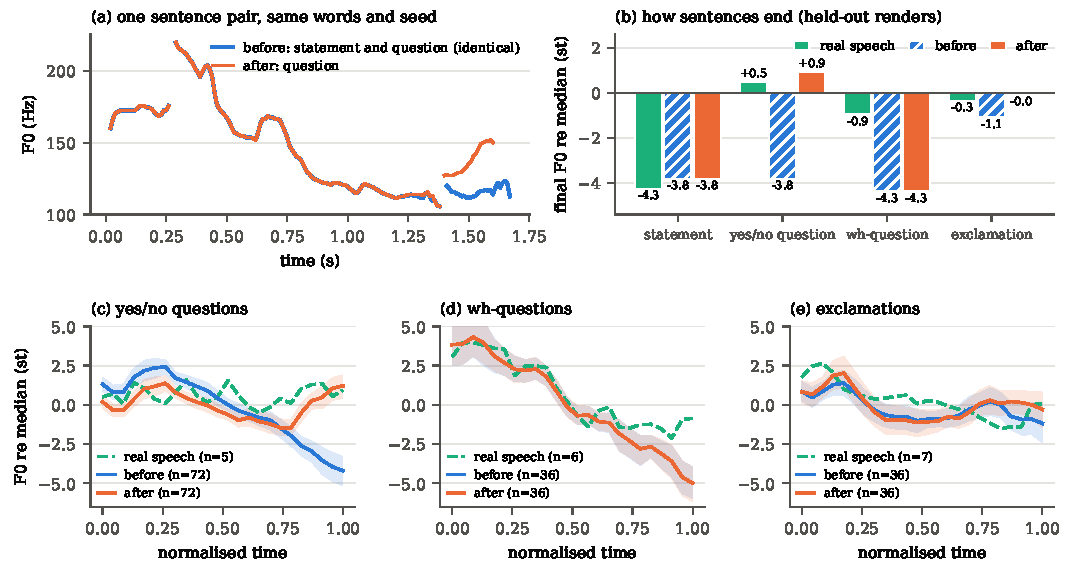
\includegraphics[width=\textwidth]{figures/fig_into.pdf}
\caption{Sentence-type intonation, held-out (even-numbered) sentences, three voices, two seeds. (a) One
minimal pair, same words and seed: before, the statement and the question are the same audio; after, the
question rises at the end. (b) Final F0 (last 150\,ms of voicing, st re the utterance median) by type:
real speech, before, after. (c--e) Mean time-normalised F0 contours with 95\% bootstrap bands. Wh-questions
are left unchanged: the model already accents the question word and falls, as real Persian
wh-questions do.}
\label{fig:into}
\end{figure*}

\textbf{Results.} Fig.~\ref{fig:into} and Table~\ref{tab:into}. On held-out pairs the final pitch of a
yes/no question now lies \RES{4.7}\,st above its statement twin (\RES{0.00} before; real speech
\RES{4.75}), and its last 0.3\,s rise (\RES{+6.9}\,st/s) instead of falling (\RES{$-$8.6}). Exclamations end
\RES{1.0}\,st higher, with a wider pitch range (\RES{6.5 $\to$ 7.3}\,st) and loudness range
(\RES{20.1 $\to$ 20.9}\,dB; real \RES{22.2}). No render failed that had not failed before; the consensus
error is unchanged within its CI and Whisper alone rises by \RES{1.8} points. Speaker similarity drops by
\RES{0.010}. UTMOS drops by \RES{0.24}, and a control shows that this is the cost of the signal processing,
not of the new contour: a flat +2\,st TD-PSOLA shift that leaves the contour as it was costs \RES{0.27}, and
real questions and exclamations score about the same as real statements (UTMOS \RES{2.92 / 2.88 vs.\ 2.97}).
We also tried to hide the cost by re-encoding and decoding each processed sentence with Mimi: UTMOS returns
to the original (\RES{$-$0.00}), but the round trip costs \RES{2.1} points of consensus error, \RES{11}
points of Whisper error and \RES{0.04} speaker similarity, so the engine does not use it.

\begin{table}[t]
\caption{Sentence-type intonation, held-out sentences (3 voices $\times$ 2 seeds); F0 in st re the
utterance median}\label{tab:into}
\centering
\setlength{\tabcolsep}{3pt}
\begin{tabular}{lccc}
\toprule
measure & before & after & real \\
\midrule
yes/no $-$ statement twin, final F0 & \RES{0.00} & \RES{+4.74} & \RES{+4.75} \\
\quad 95\% CI over pairs & & \RES{[3.99, 5.49]} & \\
yes/no, final F0 & \RES{$-$3.81} & \RES{+0.92} & \RES{+0.49} \\
yes/no, final slope (st/s) & \RES{$-$8.6} & \RES{+6.9} & \RES{+8.1} \\
exclamation, final F0 & \RES{$-$1.07} & \RES{$-$0.05} & \RES{$-$0.35} \\
wh-question, F0 on the wh-word & \RES{+3.4} & unchanged & \RES{+3.8} \\
\midrule
\multicolumn{4}{l}{\emph{quality, yes/no questions + exclamations (126 renders)}} \\
consensus CER & \RES{.019} & \RES{.021} & \\
\quad change [CI] & & \RES{+.002 [$-$.004, +.008]} & \\
failed renders & \RES{0} & \RES{0} & \\
CER, Whisper only & \RES{.173} & \RES{.191} & \\
UTMOS & \RES{3.30} & \RES{3.06} & \\
speaker similarity & \RES{.271} & \RES{.261} & \\
\multicolumn{4}{l}{\emph{controls (all 324 question/exclamation renders): UTMOS change}} \\
flat +2\,st TD-PSOLA, contour kept & & \RES{$-$0.27} & \\
rule + Mimi round trip & & \RES{$-$0.00} & \\
\bottomrule
\end{tabular}
\end{table}

\textbf{What did not work.} Before the rule we looked for a pitch direction inside the model. A linear
map from one Mimi latent frame to its F0 explains \RES{30\%} of the variance, but pushing the last frames
along it changed nothing up to three units and then broke the sound; the latent displacement of a real
$\pm$4\,st pitch shift is not a consistent direction (\RES{$R^2<0.07$}; the $+$ and $-$ shifts even point
partly the same way, cosine \RES{+0.38}). Unlike the backbone steering of \cite{vigneaux2026tunes}, the
continuous codec latents of this model offer no linear handle on pitch.

\section{Expressive prosody through the voice prompt}\label{sec:d}
\textbf{What the rule leaves flat.} Heard as whole answers, questions, surprise and loudness still barely
change from sentence to sentence. Four measurements agree. (i)~\emph{A recogniser as listener:} Whisper
writes punctuation, and for a yes/no question without a question particle the words give it no clue, so
ending its transcript with \fa{«؟»} means it heard a question. On such questions in expressive real speech
(ShEMO radio plays \cite{shemo2019}) it does so in \RES{39\%} (\RES{12/31}), in read speech (GPTInformal)
in \RES{5\%} (\RES{1/19}); our held-out renders reach \RES{3\%} without a rule and \RES{4\%} with the rule
of Sec.~\ref{sec:c}, the level of the statements (\RES{3\%}). (ii)~\emph{Energy:} in ShEMO the second half
of an utterance is \RES{4.0}\,dB below the first when neutral but only \RES{1.8} when surprised and
\RES{0.6} when happy; renders decay by \RES{5.7}\,dB, and the exclamation rule of Sec.~\ref{sec:c}, which
raised the first half, makes it \RES{7.3}. (iii)~\emph{Wh-questions} end level in real speech (\RES{$-$0.9}
to \RES{$-$1.4}\,st) but fall like statements in ours (\RES{$-$4.4}). (iv)~\emph{Clarity:} reshaping a whole
exclamation by TD-PSOLA costs \RES{0.24} UTMOS; that roughness is what a listener hears as a less clear voice.
Alternative questions (\fa{«چای یا قهوه؟»}) fall in Persian, yet that rule made them rise (\RES{+2.7}\,st).

\textbf{The prompt carries register and range.} The model continues its prompt, so we let the prompt do
the expressive part. The self-extension of Sec.~\ref{sec:b} is decoded, its F0 is raised by $r$\,st and its
excursions are scaled by $k$ (TD-PSOLA), its level is raised by $g$\,dB, and it is encoded back with the
Mimi encoder. A sentence is then generated from the clip followed by this \emph{styled} extension; only the
prompt was processed, the take is generated and decoded as before. On 108 development renders the take's
register follows the prompt's (Fig.~\ref{fig:expr}a; a quarter to all of the shift, least for the female
voice), and $(r,k,g)=(4,1.6,4)$
widens the take's pitch range from \RES{9.0} to \RES{12.2}\,st with consensus error, UTMOS, DNSMOS SIG
\cite{dnsmos2022} and speaker similarity unchanged (\RES{$-$0.001}, \RES{+0.07}, \RES{+0.01},
\RES{$-$0.001}); a decode--encode round trip alone moves register by at most \RES{0.5}\,st. Stronger
styling ($5,1.5,6$) begins to cost intelligibility and UTMOS, and on the female voice even $r=4$ cost
UTMOS on exclamations (\RES{$-$0.40} vs.\ \RES{$-$0.12} at $r=2$), so a voice whose extension has a median
F0 above 165\,Hz gets half the register shift. Exclamations and surprised questions use this
\emph{lively} prompt; a milder one for all questions ($2,1.25,2$) widened the pitch range and so deepened the
fall before the final rise (yes/no heard as questions \RES{12\%}$\to$\RES{7\%}, wh-questions fell deeper)
and was dropped. The styled prompt is built once per voice in \RES{0.5}\,s.

\textbf{The rule keeps only what a prompt cannot give: the ending.} The front end now tells apart yes/no
questions (with tag questions), wh-questions, alternative questions (left alone), surprised or echo
questions (\fa{«جدی؟»}, \fa{«؟!»}) and exclamations, whose intensity grows with \fa{«!!»}, interjections and
exclamative \fa{«چه ...!»}. A yes/no question rises over its last syllable only --- from the energy valley
before the last vowel nucleus, shape $u^{1.3}$, to 9\,st above the median --- and that syllable is
lengthened by 15\%; a surprised question rises to 8\,st; a wh-question's or an exclamation's final fall stops
at $-1$\,st; the second half of questions and exclamations is raised by up to 2 and 3.5\,dB with a plain
gain envelope, as in excited speech. Over a text, exclamations get +3\,dB (times intensity), surprised
questions +2 and other questions +0.5\,dB; a paragraph's first sentence +1\,dB and its last $-$1.5. The
end height, lengthening and final-syllable energy were chosen on development sentences by the
recogniser-heard question rate against UTMOS.

\begin{figure*}[t]
\centering
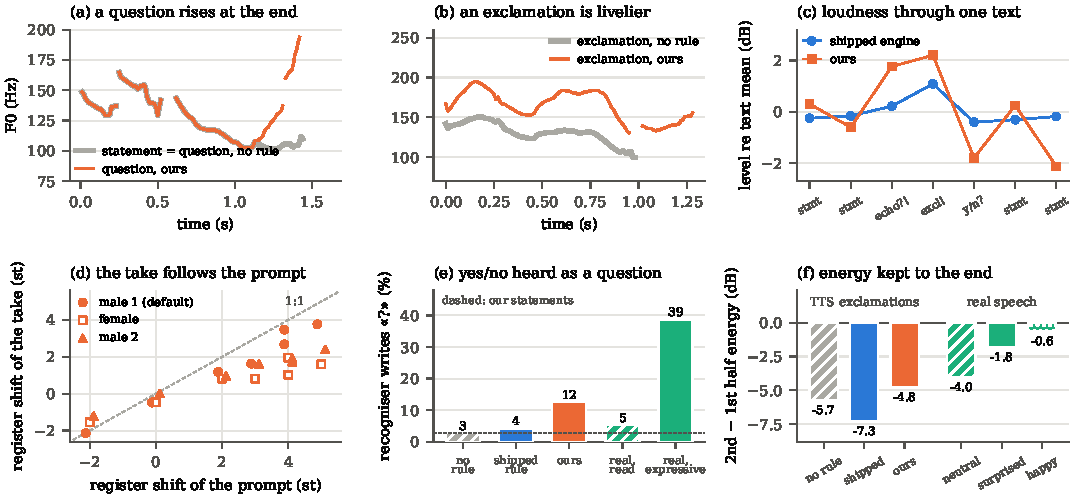
\includegraphics[width=\textwidth]{figures/fig_expr.pdf}
\caption{Expressive prosody. (a) Register of the take vs.\ register shift of the styled prompt, three voices
(the female voice transfers least). (b) Held-out yes/no questions without a question particle heard as
questions by Whisper, vs.\ real read and expressive speech; dashed: our statements. (c) Energy of the second
half of a sentence relative to the first (held-out; real: ShEMO by emotion). (d) Sentence loudness through
one text (default voice), shipped engine (Sec.~\ref{sec:c}) vs.\ this section.}
\label{fig:expr}
\end{figure*}

\begin{table}[t]
\caption{Expressive prosody, held-out sentences (3 voices $\times$ 2 seeds; 348 question and exclamation
renders) and whole texts (8 texts, 48 renders). C: rule of Sec.~\ref{sec:c}; D: this section.}\label{tab:expr}
\centering
\footnotesize
\setlength{\tabcolsep}{2.2pt}
\begin{tabular}{lccc}
\toprule
measure & no rule & C & D \\
\midrule
yes/no heard as question (\fa{«؟»}) & \RES{3\%} & \RES{4\%} & \RES{12\%} \\
tag questions heard as question & \RES{17\%} & \RES{56\%} & \RES{61\%} \\
yes/no $-$ statement, final F0 (st) & \RES{0.00} & \RES{+3.63} & \RES{+3.56} \\
alternative q., final F0 (st; falls) & \RES{$-$0.40} & \RES{+2.68} & \RES{$-$0.40} \\
wh-q., final F0 (st; real $\approx-$1) & \RES{$-$4.35} & \RES{$-$4.35} & \RES{$-$2.99} \\
surprised q., register (st) & 0 & \RES{+1.05} & \RES{+3.65} \\
exclam., register (st) & 0 & \RES{+1.46} & \RES{+1.65} \\
exclam., pitch range (st) & \RES{7.5} & \RES{7.1} & \RES{10.4} \\
exclam., level (dB) & 0 & \RES{+0.7} & \RES{+2.2} \\
exclam., 2nd$-$1st half energy (dB) & \RES{$-$5.7} & \RES{$-$7.3} & \RES{$-$4.8} \\
texts: sentence level SD (dB) & \RES{0.49} & \RES{0.67} & \RES{1.31} \\
texts: sentence register SD (st) & \RES{1.22} & \RES{1.20} & \RES{1.61} \\
\midrule
consensus CER (failed renders) & \RES{.041 (9)} & \RES{.043 (10)} & \RES{.041 (8)} \\
$\Delta$UTMOS, all / exclam. & & \RES{$-$.12/$-$.24} & \RES{$-$.10/$-$.02} \\
$\Delta$DNSMOS SIG & & \RES{$-$.028} & \RES{$-$.040} \\
$\Delta$speaker similarity & & \RES{$-$.002} & \RES{$-$.009} \\
texts, D$-$C: CER/UTMOS/SIG & & & \RES{$-$.001/$-$.03/+.00} \\
\bottomrule
\end{tabular}
\end{table}

\textbf{Results.} Table~\ref{tab:expr}. On held-out sentences, yes/no questions are now heard as questions
three times as often as with the rule of Sec.~\ref{sec:c} (\RES{12\%} vs.\ \RES{4\%}; real read speech
\RES{5\%}, expressive \RES{39\%}) at the same rise over their statement twins; alternative questions keep
their fall; wh-questions end \RES{1.4}\,st higher, toward real speech; surprised questions are spoken
\RES{3.7}\,st higher and \RES{1.9}\,dB louder; exclamations come out with a \RES{38\%} wider pitch range,
\RES{2.2}\,dB louder, with energy kept up to the end (\RES{$-$4.8}\,dB, between real neutral and excited
speech), at almost no UTMOS cost (\RES{$-$0.02}, against \RES{$-$0.24} for the old rule). Over whole texts
the loudness of consecutive sentences varies twice as much (SD \RES{0.67}$\to$\RES{1.31}\,dB; real read speech
\RES{1.52}) and register \RES{34\%} more. Intelligibility is unchanged (consensus error \RES{.041}, failed
renders \RES{8} vs.\ \RES{9}); the costs are a small loss of speaker similarity on exclamations
(\RES{$-$0.028}) and UTMOS on surprised one- and two-word questions (\RES{$-$0.25}), where the rise and the
prompt both act on very little audio.

\textbf{What did not work.} Pitch marks from zero-frequency filtering \cite{zff2008} made TD-PSOLA rougher on
codec speech (flat +2\,st shift: UTMOS \RES{$-$0.37} vs.\ \RES{$-$0.27}). Undoing the energy decay of the last
syllable only amplified its creak (UTMOS \RES{$-$0.05} at 3\,dB, \RES{$-$0.14} at 6\,dB). For clarity, the default
voice renders \RES{10}\,dB weaker at 2.5--6\,kHz than its own clip, but an equaliser that moves each render's
long-term spectrum toward the clip lowered UTMOS (\RES{$-$0.06}) and DNSMOS SIG (\RES{$-$0.06}); equalising
the prompt instead brightened the take by \RES{4.5}\,dB but cost speaker similarity (\RES{$-$0.015}). Neither
is used: the clarity gain that holds up is removing the whole-sentence processing from exclamations.

\section{Discussion and limitations}
\textbf{Why the ending matters.} The training cut makes the prompt the audio \emph{before} the target, so
the model learns to continue from wherever the prompt stops. A prompt that stops on a completed sentence
asks for a new one; a prompt that stops mid-phrase --- a tightly trimmed clip, a clip after an extension, an
extension cut short --- asks the model to finish something it was not given the words for, and the result
is a replay of the prompt or a short target with its ending dropped. Self-extension is one way to make every
voice end the same, well-formed way without asking users for longer or pause-padded recordings; padding the
clip with silence alone was inconsistent across voices in our probes.

\textbf{What a punctuation-blind model can and cannot learn.} The model reproduced every intonation cue
that the \emph{words} carry --- the accent on a question word, the fall after it --- and none that only the
mark carries. Since the front end still sees the mark, the missing cue can be put back after synthesis;
the cue is small and well documented (a final rise of about 5\,st), so a rule suffices, and its only
measured cost is that of the signal processing. The same split of labour would apply to any TTS model
trained on text from which punctuation was stripped.

\textbf{Limitations.} One model and six voice clips (three from one speaker); results may differ for discrete-token or
attention-aligned TTS. Intelligibility is measured with recognisers, which is why we report two and their
floor on real speech. A first blind A/B test (one listener, one male voice, 60 pairs) heard no difference
in preference (\RES{same 33, base 15, extension 12; sign test $p=.70$}) and marked word errors in \RES{7 base
and 5 extended} renders (\RES{3 vs.\ 1} on Persian-only sentences), but its error marks and the
recognisers' failures fell on different takes (\RES{0 of 21 in common}); the intelligibility gains above
are therefore recogniser-measured and await a larger listening test. The
extension sentence is a hyperparameter: of seven candidates two helped both voices, no simple property
predicted which, and we fixed it on development data. English sentences, read through mapped Persian phonemes, did not benefit from a Persian
extension (acronym cases drifted, \RES{6.1\% $\to$ 12.1\%}, n.s.); keeping the plain clip for sentences the
front end marks as English removes this (\RES{6.1\%}, identical renders), so the engine extends the prompt
for Persian and code-mixed sentences only. The extension changes the prosody of every unit, not only short
ones; we measured joins and UTMOS but not long-form drift. The intonation targets come from one real
speaker and the literature; the exclamation rule rests on a small reference (\RES{7} utterances) and is a
design choice rather than a measured norm; intonation is evaluated by F0 measurements, not yet by
listeners; the TD-PSOLA processing costs \RES{0.24} UTMOS, which a codec round trip hides only at a cost in
intelligibility; and a rule cannot produce question prosody that differs in timing or voice quality.
The expressive results of Sec.~\ref{sec:d} rest on acoustic measurements and on one recogniser used as a
listener, whose question rate on real expressive speech is itself only \RES{39\%}; the expressive reference
(ShEMO) is acted radio speech whose texts we attached by recogniser matching (\RES{279} of \RES{760} clips)
and which carries no speaker labels, so its register cannot be compared across emotions; the style
strengths and the half shift for high voices were chosen on few development renders; and surprised one- and
two-word questions still lose \RES{0.25} UTMOS. A listening test of the whole pipeline is the next step.

\section{Conclusion}
Short inputs are where a small CPU TTS model fails, and a single ASR judge overstates how often. Signals
available without a recogniser locate risky units but not failed takes, so retries without a recogniser
mostly add cost. Making the voice prompt end the way training prompts end --- with the model's own reading of
one neutral sentence after the clip --- halves failed short renders on held-out data, rescues clips that
are cut mid-utterance, raises UTMOS, smooths chunk joins and costs nothing per request; it lets the engine drop its retries, halving the generation work
while making fewer errors. Its price, a small loss of speaker similarity for one of three voices, disappears when the
extension take is chosen by speaker similarity, at part of the intelligibility gain. Finally, the model
reads every yes/no question as a statement because it never sees punctuation; a contour rule driven by the
written mark and applied by TD-PSOLA gives held-out questions the final rise of real speech (\RES{+4.7}\,st
over their statement twins) without new recognition failures, at the UTMOS cost of the signal processing.
Because the voice prompt carries register and pitch range, the rest of expressive delivery can come from the
model itself: a re-pitched, widened copy of its own reading makes exclamations and surprise livelier with
almost no quality cost, the audio rule shrinks to the sentence endings and the energy, and the loudness of a
text now changes from sentence to sentence as speech does.
Code,
sentence sets and labels will be released with the paper \RES{[URL]}.

\bibliographystyle{IEEEtran}
\bibliography{refs}
\end{document}
